\hypertarget{gausspoint_8h}{
\section{src/gausspoint.h File Reference}
\label{gausspoint_8h}\index{src/gausspoint.h@{src/gausspoint.h}}
}
Point for numerical integration. 

{\tt \#include $<$vector$>$}\par
{\tt \#include $<$map$>$}\par
{\tt \#include \char`\"{}node.h\char`\"{}}\par
{\tt \#include \char`\"{}common.h\char`\"{}}\par
{\tt \#include \char`\"{}material.h\char`\"{}}\par


Include dependency graph for gausspoint.h:\nopagebreak
\begin{figure}[H]
\begin{center}
\leavevmode
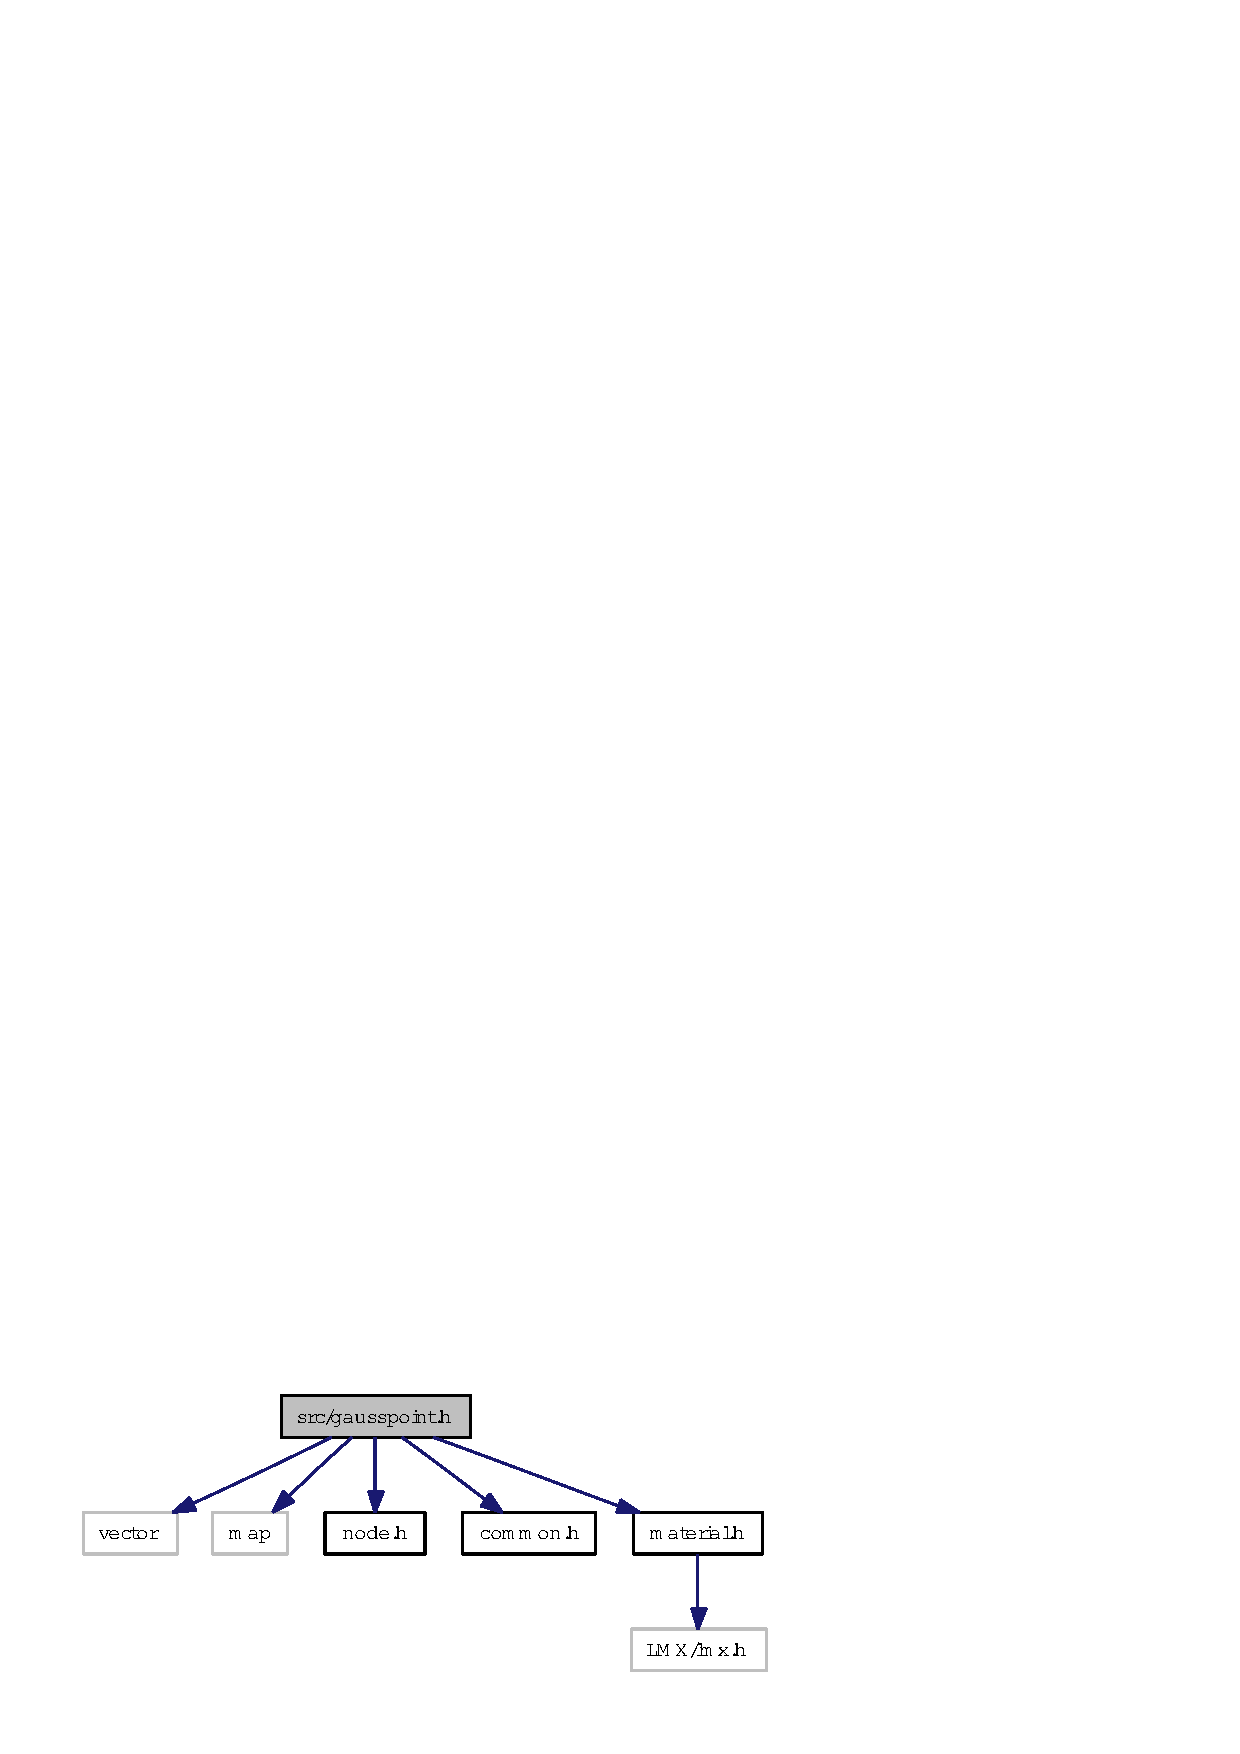
\includegraphics[width=185pt]{gausspoint_8h__incl}
\end{center}
\end{figure}


This graph shows which files directly or indirectly include this file:\subsection*{Namespaces}
\begin{CompactItemize}
\item 
namespace \hyperlink{namespacemknix}{mknix}
\end{CompactItemize}
\subsection*{Classes}
\begin{CompactItemize}
\item 
class \hyperlink{classmknix_1_1GaussPoint}{mknix::GaussPoint}
\end{CompactItemize}


\subsection{Detailed Description}
Point for numerical integration. 

\begin{Desc}
\item[Author:]Daniel Iglesias Ib��ez \end{Desc}


Definition in file \hyperlink{gausspoint_8h-source}{gausspoint.h}.